\chapter{Results}
{\samenvatting todo}
\section{Person specific}
At first research was done in a person specific setting. This means that that algorithm was trained on several samples from a single person, before it was tested on the same person.
This section will go over the results.

\npar

The first step was to transform the continuous valence and arousal values to classes. This was done by performing a simple binary classification. Given that the dimension range from 1 to 9, all labels with a valence or arousal below 5 were reported as low valence or arousal respectively. The remaining valence or arousal were placed in the high valence or arousal respectively.

\section{Used approach}

This thesis compares the aforementioned features and the aforementioned feature selection methods. For this a two stepped algorithm, inspired by the advanced random forest method, explained in Section \ref{rfmethod}, was used. In short, the first step is to rank all the features and only take the top X of the features. This threshold is applied to limit computation times and throw out features that have very low importance. The next step is to iteratively build a model by selecting features out of the remaining feature set. This approach is depicted in Figure \ref{flow}.

\mijnfiguur{width=0.9\textwidth}{flow}{The used approach of this thesis.}

As you can see in Figure \ref{flow}, the approach starts by separating a test set to evaluate the final performance of the algorithm. This test set contained 10 of the 40 samples. Next, the aforementioned feature selection methods are applied to the train set. A top $X$ of the features is then kept.

\npar

In the next step different models are build. This is done iteratively by starting with an empty feature set. In the add step, a feature is added to this set and the cross validation error is determined. Cross validation is a technique that separates the data in N folds, as shown in Figure \ref{CVscheme}. Next the algorithm is trained on N-1 blocks and tested on the remaining blocks. This is done N times and the average of the performance is then reported as cross validation error. 

%CV fig
\mijnfiguur{width=0.55\textwidth}{CVscheme}{Cross validation}

The advantage of using a cross validation scheme is that it gives a pretty good estimation of the generalisation of the algorithm, while still using all train data. This step is important because it ensure that the chosen features have good generalisation properties. Good feature should perform well on unseen samples. Note that the test set, displayed in red is not used during cross validation. The test set is kept completely separate to ensure that a fair estimate of the generalisation is achieved.

\npar

Next the average of the cross validation errors and the standard deviation is calculated. The average cross validation minus the standard deviation is b
then compared to the previous best performance. If the performance is better, the feature is kept in the feature set. If the performance is not better, the feature is neglected. The standard deviation is included to increase the stability of the algorithm. By making sure that the new model performs better in a statistical way, one can avoid that small differences in averages lead to a different model.

\npar

In the final step the performance of the test set is determined by the accuracy metric. Accuracy is chosen as metric, because this metric gives a clear and intuitive measurement of performance.

\npar

%params
The first parameter of this flow is the threshold parameter, indicated in the figure as $X$. This threshold cancels features with low importance, by simply taking the best $X$ features from the feature ranking. Assigning a high value to the threshold will increase calculation times as more features are available for the building phase. The performance of the model, will not be better, since a lot of the additional features will have low importance values. Setting a low threshold is also not good, as this might cancel out important features. 

\npar

In this work, the parameter was fixed to 30 for all feature selection methods for the following reasons. First, considering that there are 30 samples in the feature set, having 30 features is already more than enough. Note that a well-known rule of thumb is to have at least 10 times more samples than features\citep{rot1,rot2}\footnote{Note that this is just a rule of thumb, and therefore not proven theoretically. In practice however, it turns out to work quite well.}. Second, looking at the features that were selected during training, one can see that usually around 5-7 features remain. The last selected feature usually has a rank around 20, meaning that the last 10 available features in the building phase are rarely used.

\npar

A second parameter of this model is a model to estimate the performance. For this, two different models were compared. The first model is an SVM with a radial basis functions kernel. This model was chose because it has proven itself in multiple emotion recognition studies. Additionally, SVM are capable to handle small dataset, which gives this method an advantage in this experiment. The next model is a random forest with 2000 estimators. This model was mainly chosen, because feature selection with random forest deliver good results, according to literature\citep{rfPaper}. Using the same algorithm in both feature selection and building phase, means that the algorithm can select its own features. In other words features that work well for the specific algorithm are more likely to be chosen as this is done by the same algorithm.

\subsection{Comparing the different models}

\subsection{Comparing the different feature selection methods}

When looking at the accuracies of the different feature selection models in combination with the SVM, it becomes quickly clear that the results are statistically equivalent. 

The corresponding feature selection method for each bar in Figure \ref{accComp_arousalSVM} and Figure \ref{accComp_valenceSVM} are shown in Table \ref{accCompLbl} below.

\mijnfiguur{width=0.9\textwidth}{accComp_arousalSVM}{Comparison of different feature selection methods for arousal recognition. The blue bars correspond to filter selection methods. Red bars correspond to wrapper methods and green bars are used for the embedded methods.}

\mijnfiguur{width=0.9\textwidth}{accComp_valenceSVM}{Comparison of different feature selection methods for valence recognition. The blue bars correspond to filter selection methods. Red bars correspond to wrapper methods and green bars are used for the embedded methods.}

\begin{table}[H]
\centering
\begin{tabular}{ll|ll}
\textbf{number} & \textbf{Feature selection method} & Number & Feature selection method \\
\textbf{0}      & Pearson                           & \textbf{6}      & LDA                      \\
\textbf{1}      & Mutual information                & \textbf{7}      & Lasso regression         \\
\textbf{2}      & Distance correlation              & \textbf{8}      & Ridge regression         \\
\textbf{3}      & ANOVA                             & \textbf{9}      & Random forests           \\
\textbf{4}      & Linear regression                 & \textbf{10}     & PCA                      \\
\textbf{5}      & SVM                      &        &                         
\end{tabular}
\caption{The different feature selection methods and their labels\label{accCompLbl}.}
\end{table}

From a statistical point of view, all these methods are equivalent in performance. However it is important to note that some of these methods %TODO

%The next discussion will focus mainly on the random forest for feature selection. this is done for three reasons. First, this method is the most proven method in literature. Second, the selected features agree with most of the literature. Third, this method is the most advanced, meaning that it is one of the few methods that is able to find combinations of features that work well. 

\clearpage

\subsection{Selected features}

To compare which features where chosen, the feature set was divided into 9 categories:
\begin{enumerate}
\item \textbf{Power features:} PSD and FE features of a single channel
\item \textbf{Asymmetry features:} DASM, RASM, DCAU and RCAU features that represent a the (a)symmetry between two channels.
\item \textbf{Fractions:} Alpha/beta and fractions of different power ratios of a channels.

\item \textbf{Heart rate:} the statistical values of the heart rate.
\item \textbf{Galvanic skin response:} the statistical values of the GSR.
\item \textbf{Respiration:} the statistical values of the respiration.
\item \textbf{Bloop pressure:} the statistical values of the plethysmograph.
\item \textbf{Skin temp:} the statistical values of the skin temperature.
\end{enumerate} 

The results for arousal are depicted in Figure \ref{arousalpies}, the legend is shown in Figure \ref{arousalpieslegend}. When looking at the different selected features for the different feature seleciton methods, it becomes clear that the most valuable features are the asymmetry features combined with the power features.

\npar

One can easily see that the amount of asymmetry features is always the highest, except in case of linear, mutual information and lasso regression. This can be explained by the fact that these methods are not very advanced. Additionally, lasso regression is very prone to noise, as explained earlier in Section \ref{lassoregression}. 

\npar

For arousal one can thus conclude that the different feature selection methods agree mostly on what set of feature categories is relevant. The most import features are the asymmetry features, followed by the power features. The non-EEG features are rarely chose and do not seem to be of importance here. It is also important to note that the fractions of frequency bands is not as important as previously thought. Literature suggested that the fractions of the alpha versus the beta frequency band would give an indication for the arousal of a subject. The main argument for this was the fact that arousal measures how active a person is feeling. A large fraction of alpha and beta power means that the brain is in a relaxed state or in an active and focussed state respectively. Looking at these fractions was therefore supposed to give insight in the arousal. These results indicate that the asymmetry and power features are more relevant.

\begin{figure}[!tbp]
  \centering
  \caption{Selection features for arousal classification.\label{arousalpies}}
  \begin{minipage}[b]{0.3\textwidth}
    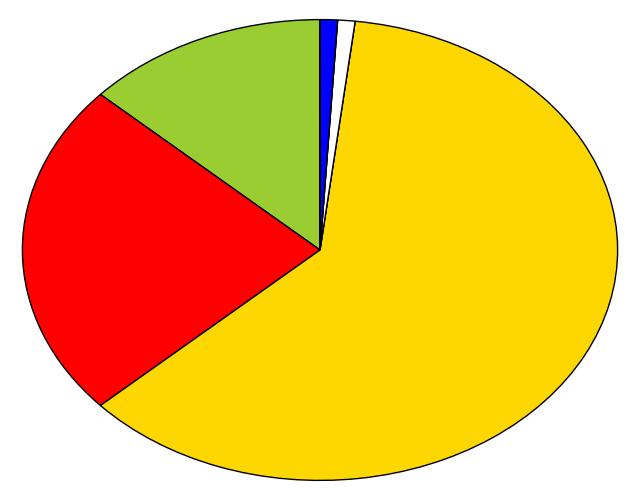
\includegraphics[width=\textwidth]{arousalALLpearsonR}
    \caption{Pearson correlation}
  \end{minipage}
  \hfill
  \begin{minipage}[b]{0.3\textwidth}
    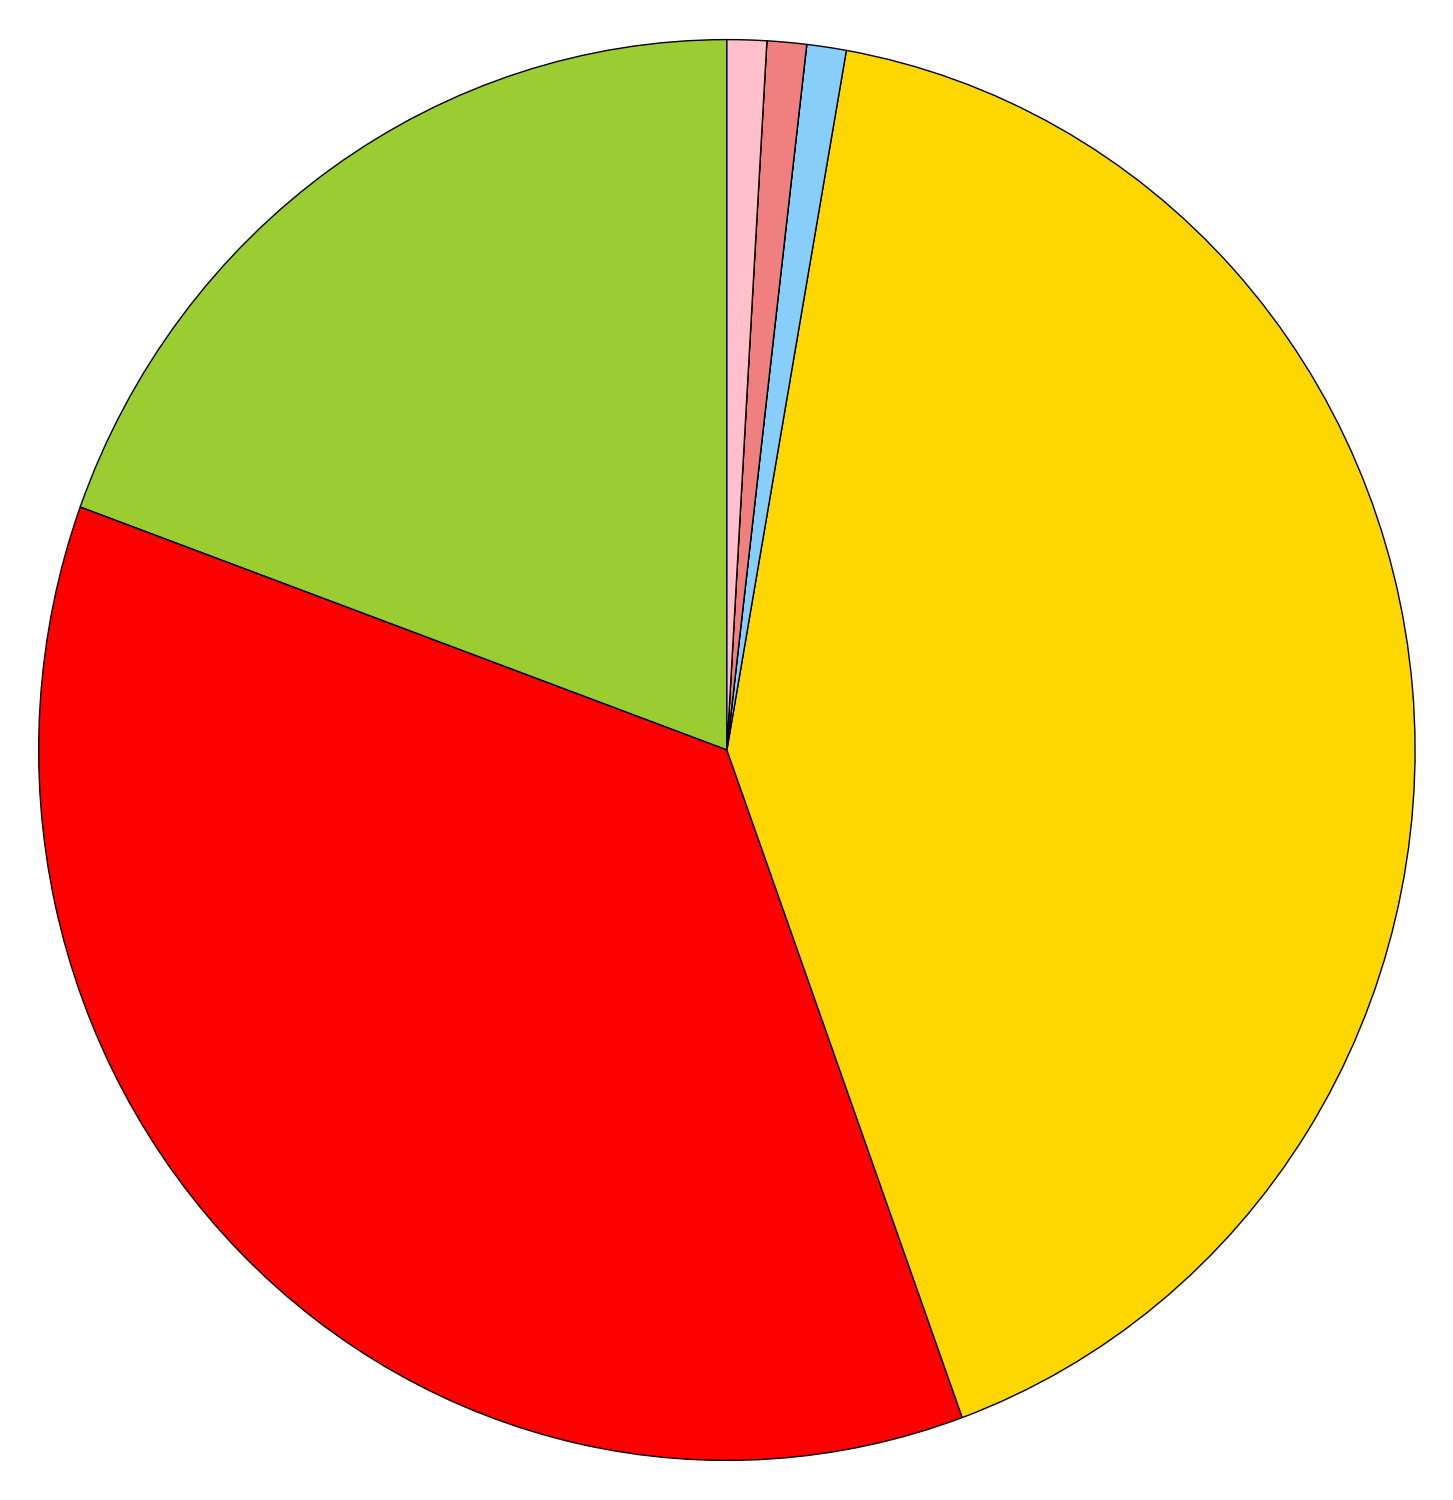
\includegraphics[width=\textwidth]{arousalALLMutInf}
    \caption{Mutual information}
  \end{minipage}
  \hfill
  \begin{minipage}[b]{0.3\textwidth}
    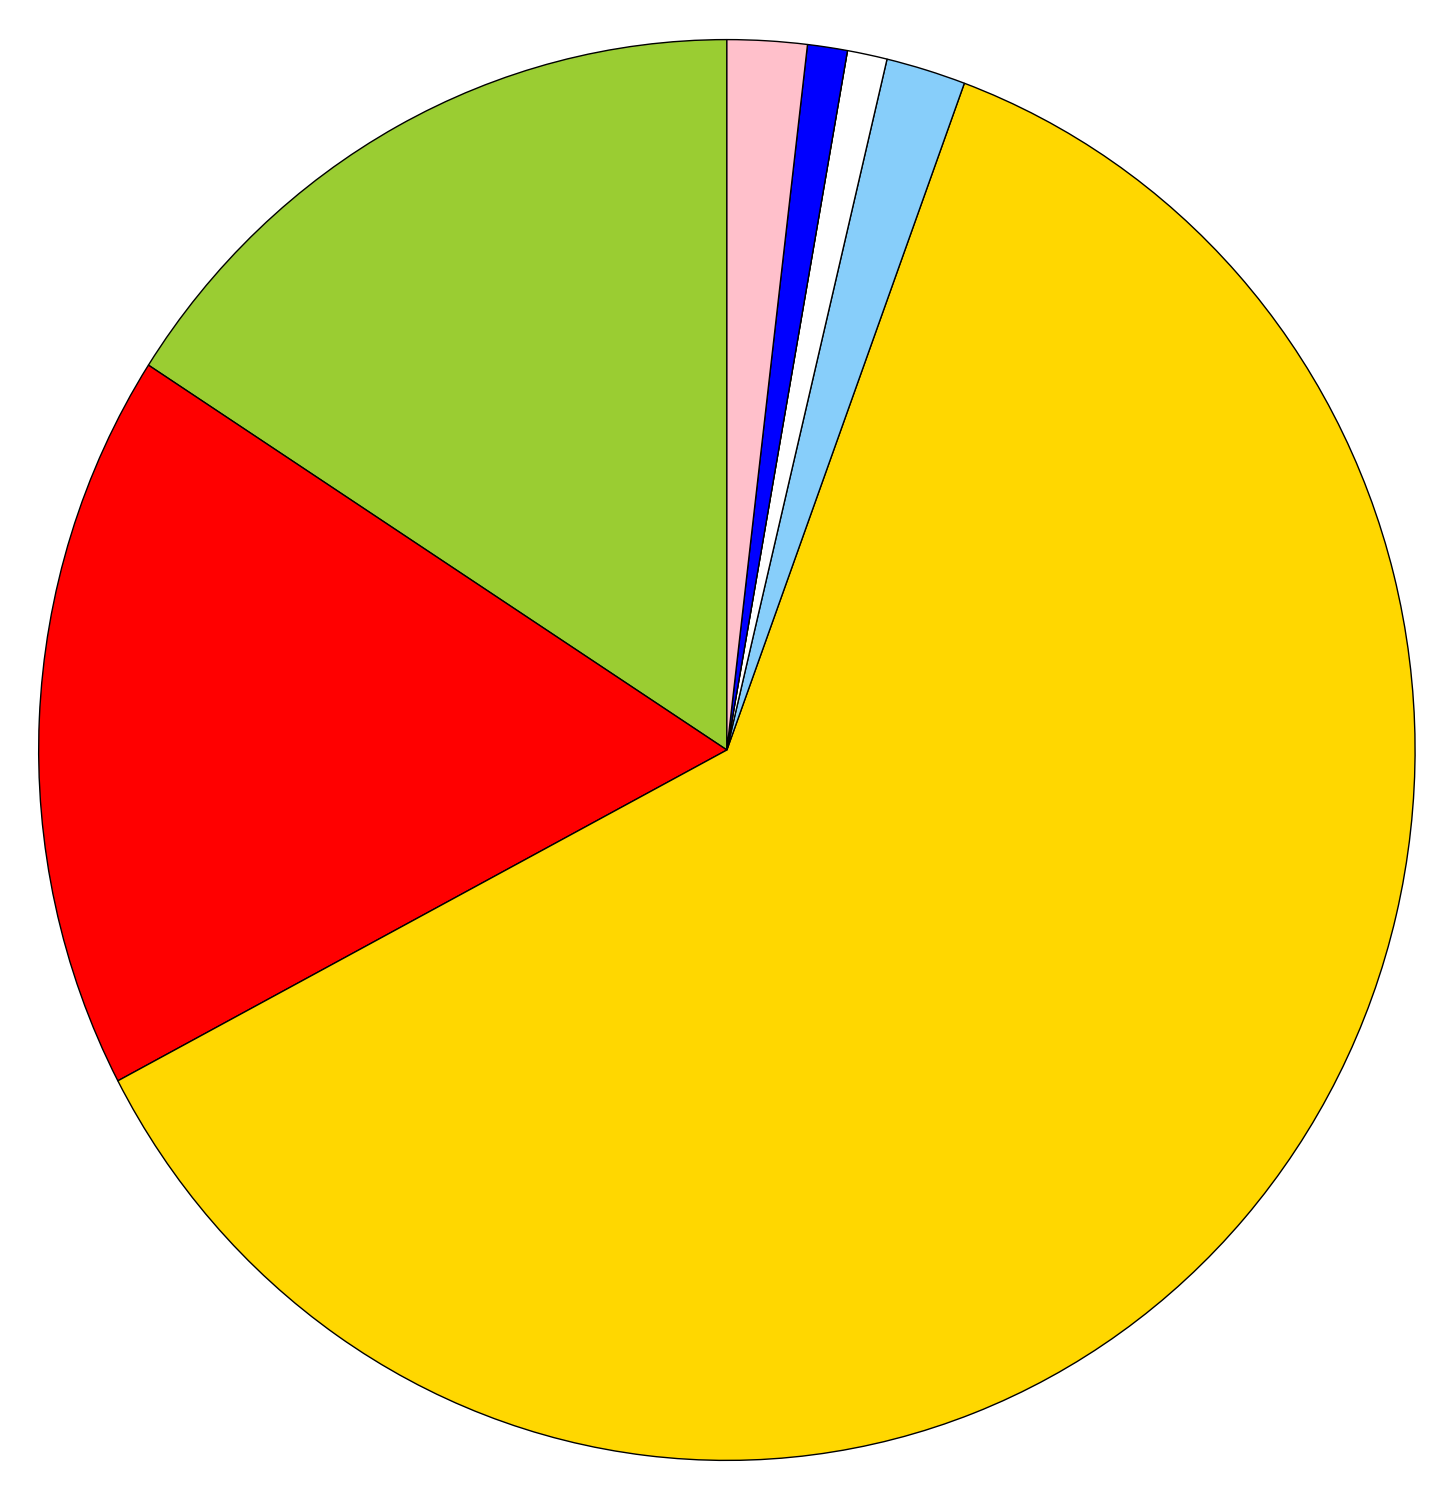
\includegraphics[width=\textwidth]{arousalALLdCorr}
    \caption{Distance Correlation}
  \end{minipage}
  
  \begin{minipage}[b]{0.3\textwidth}
    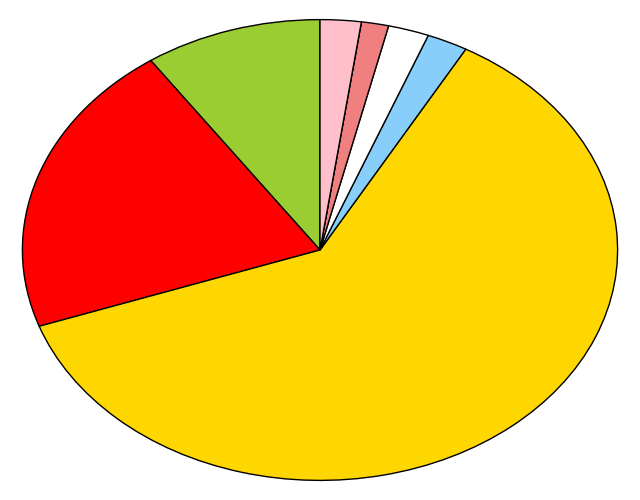
\includegraphics[width=\textwidth]{arousalALLANOVA}
    \caption{ANOVA}
  \end{minipage}
  \hfill
  \begin{minipage}[b]{0.3\textwidth}
    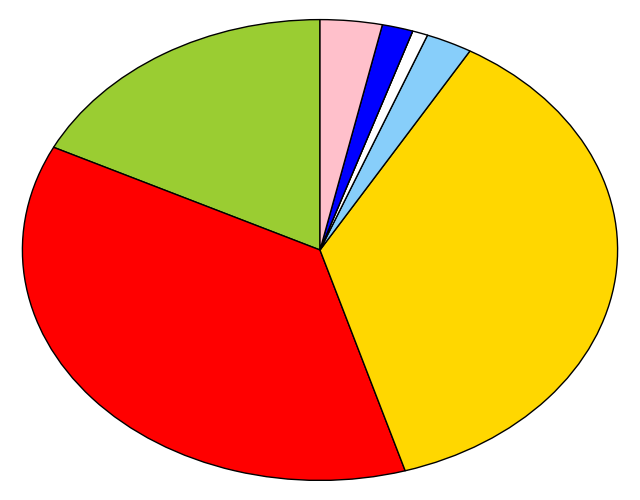
\includegraphics[width=\textwidth]{arousalALLLR}
    \caption{Linear regression}
  \end{minipage}
  \hfill
  \begin{minipage}[b]{0.3\textwidth}
    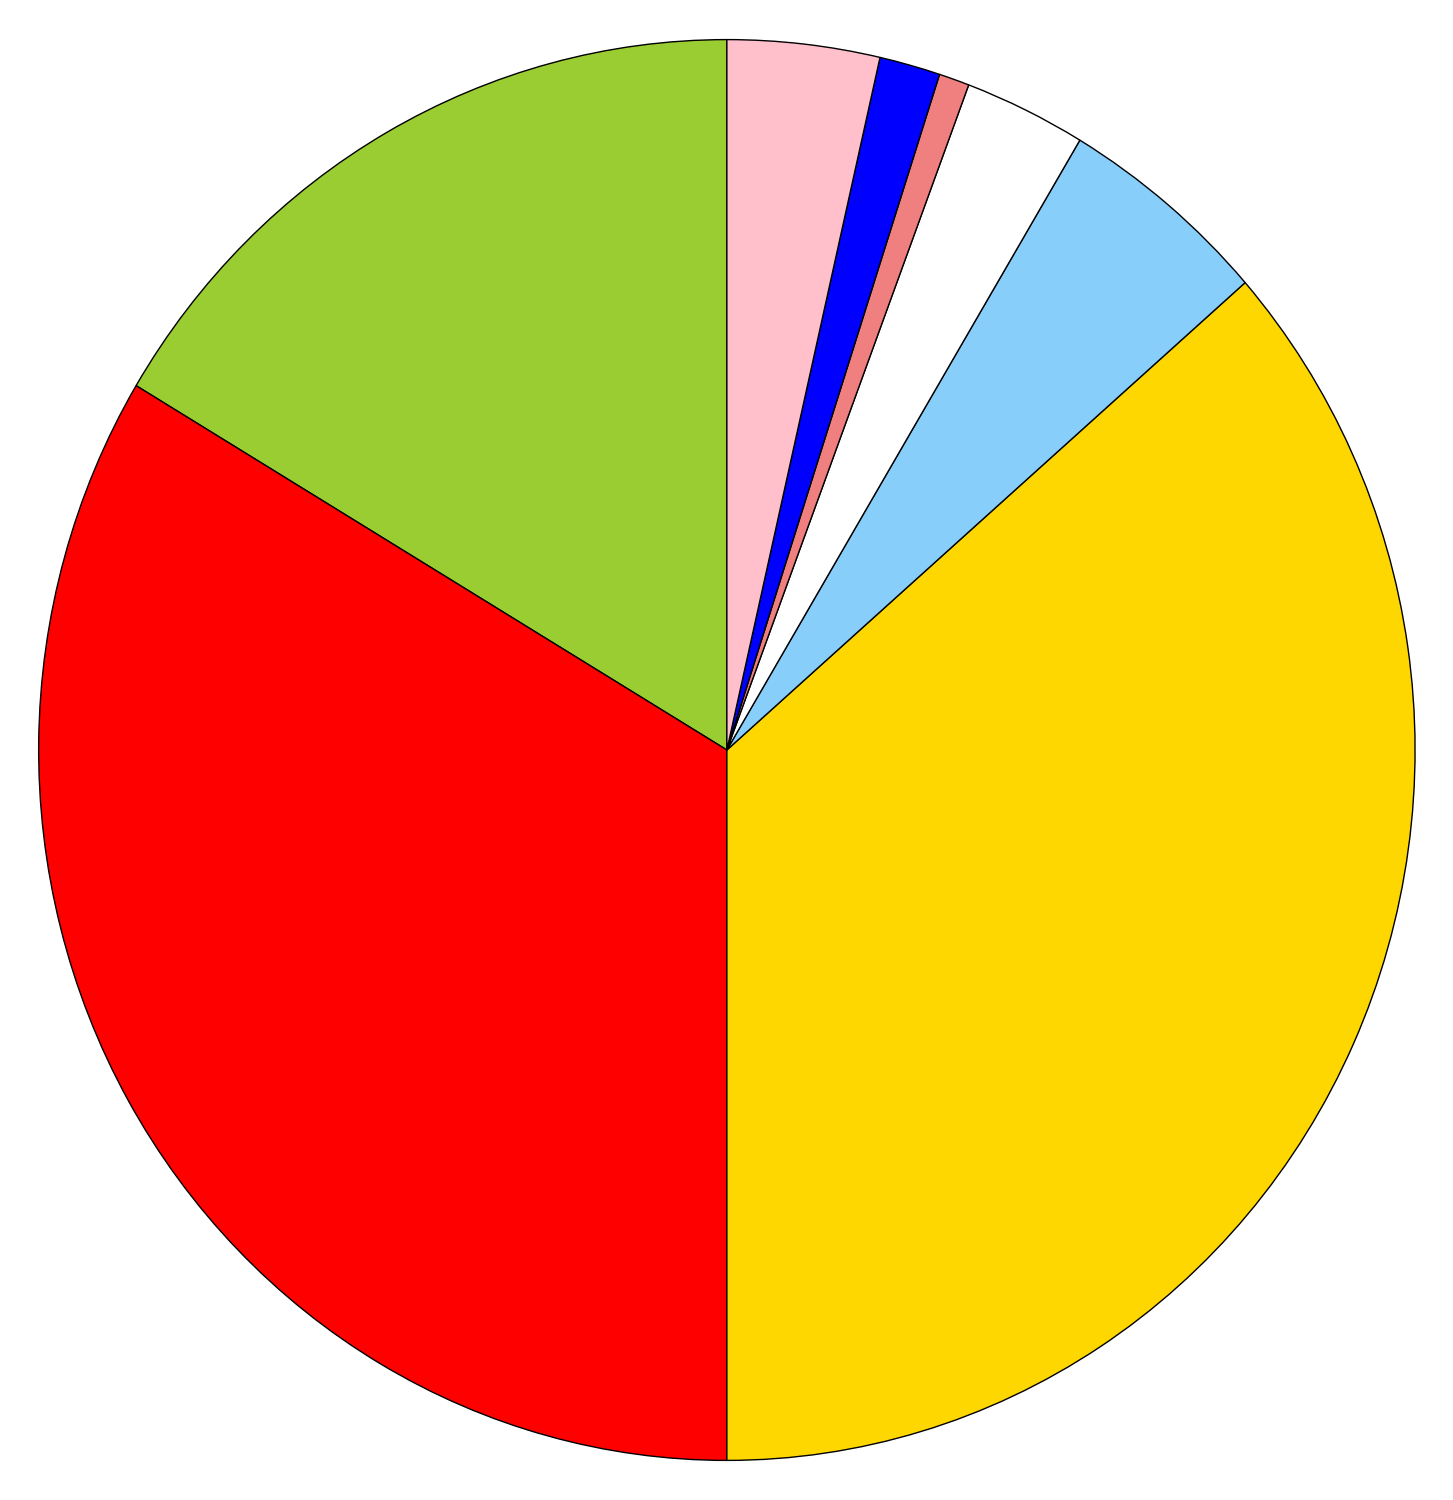
\includegraphics[width=\textwidth]{arousalALLSVM}
    \caption{SVM}
  \end{minipage}
  
  \begin{minipage}[b]{0.3\textwidth}
    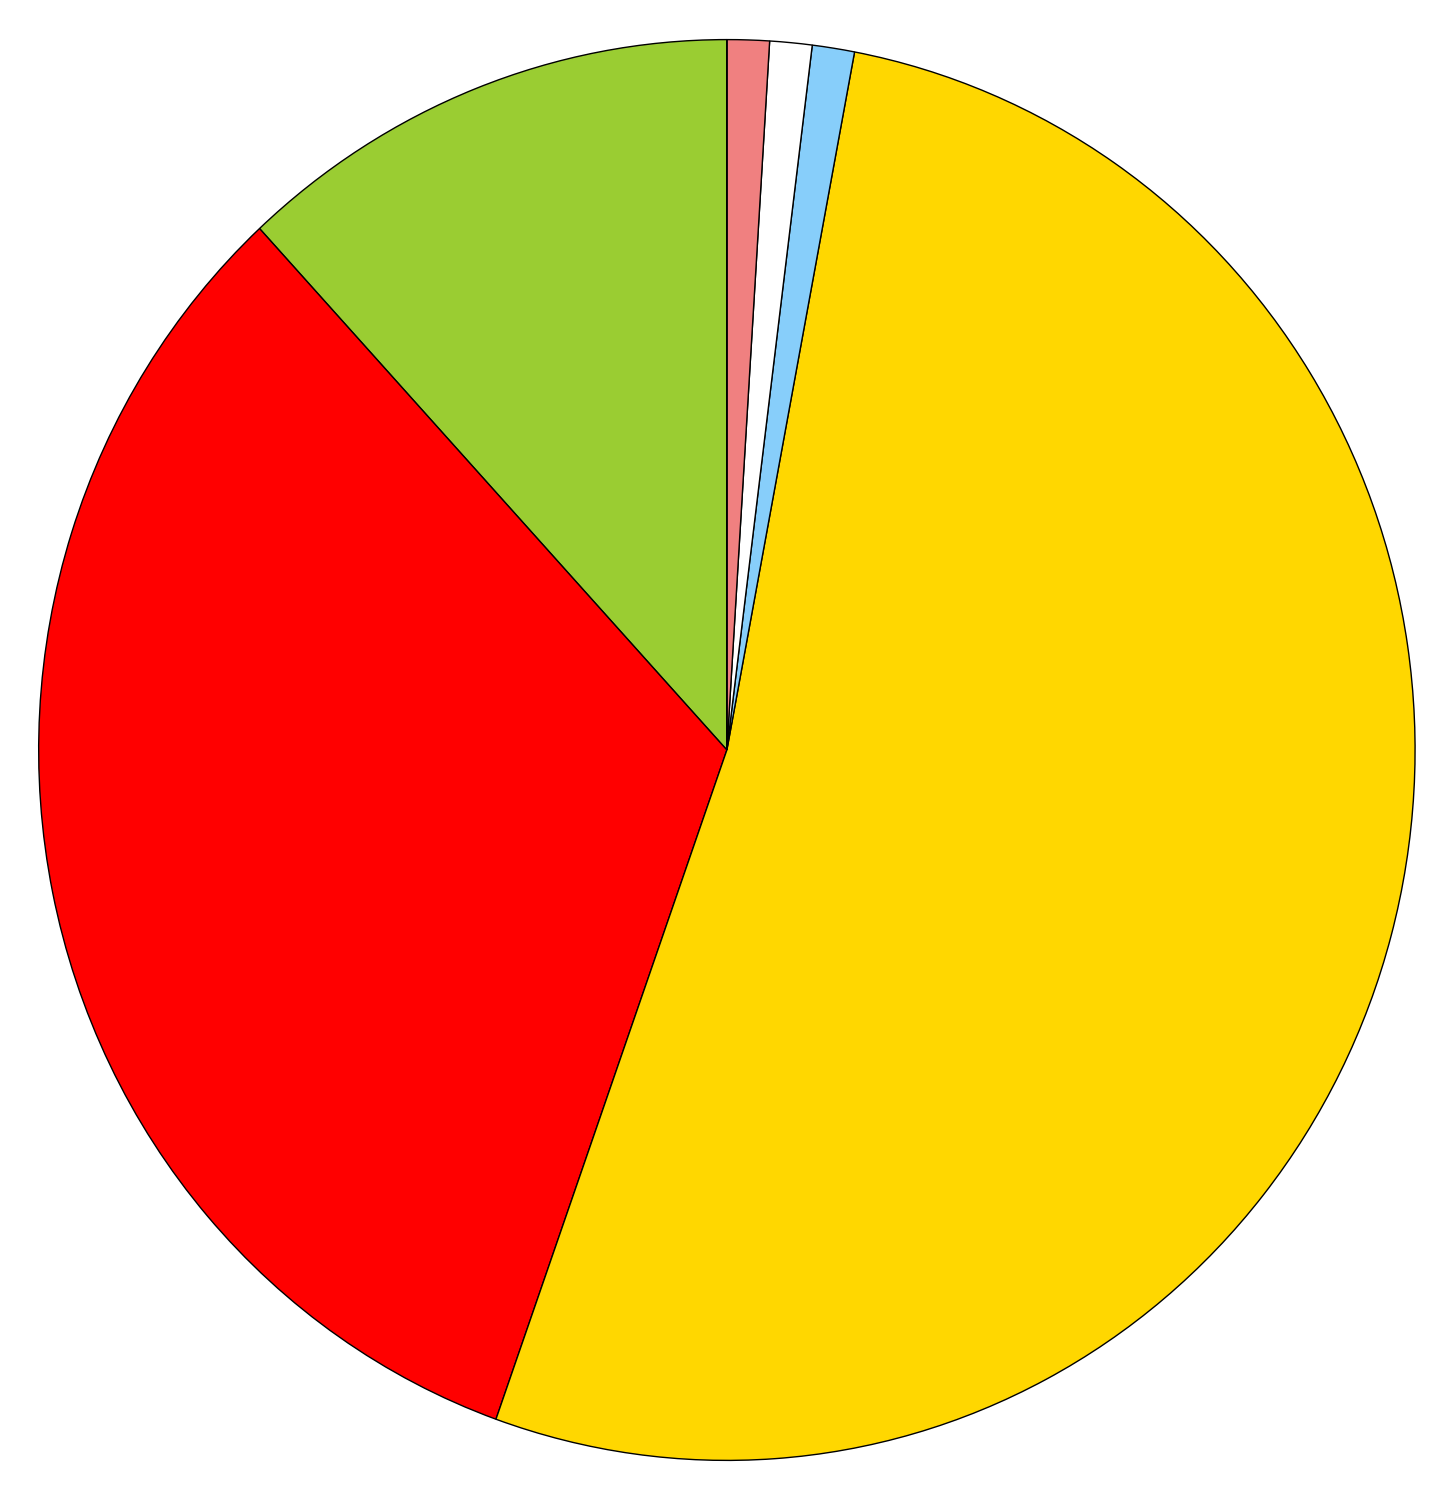
\includegraphics[width=\textwidth]{arousalALLLDA}
    \caption{LDA}
  \end{minipage}
  \hfill
  \begin{minipage}[b]{0.3\textwidth}
    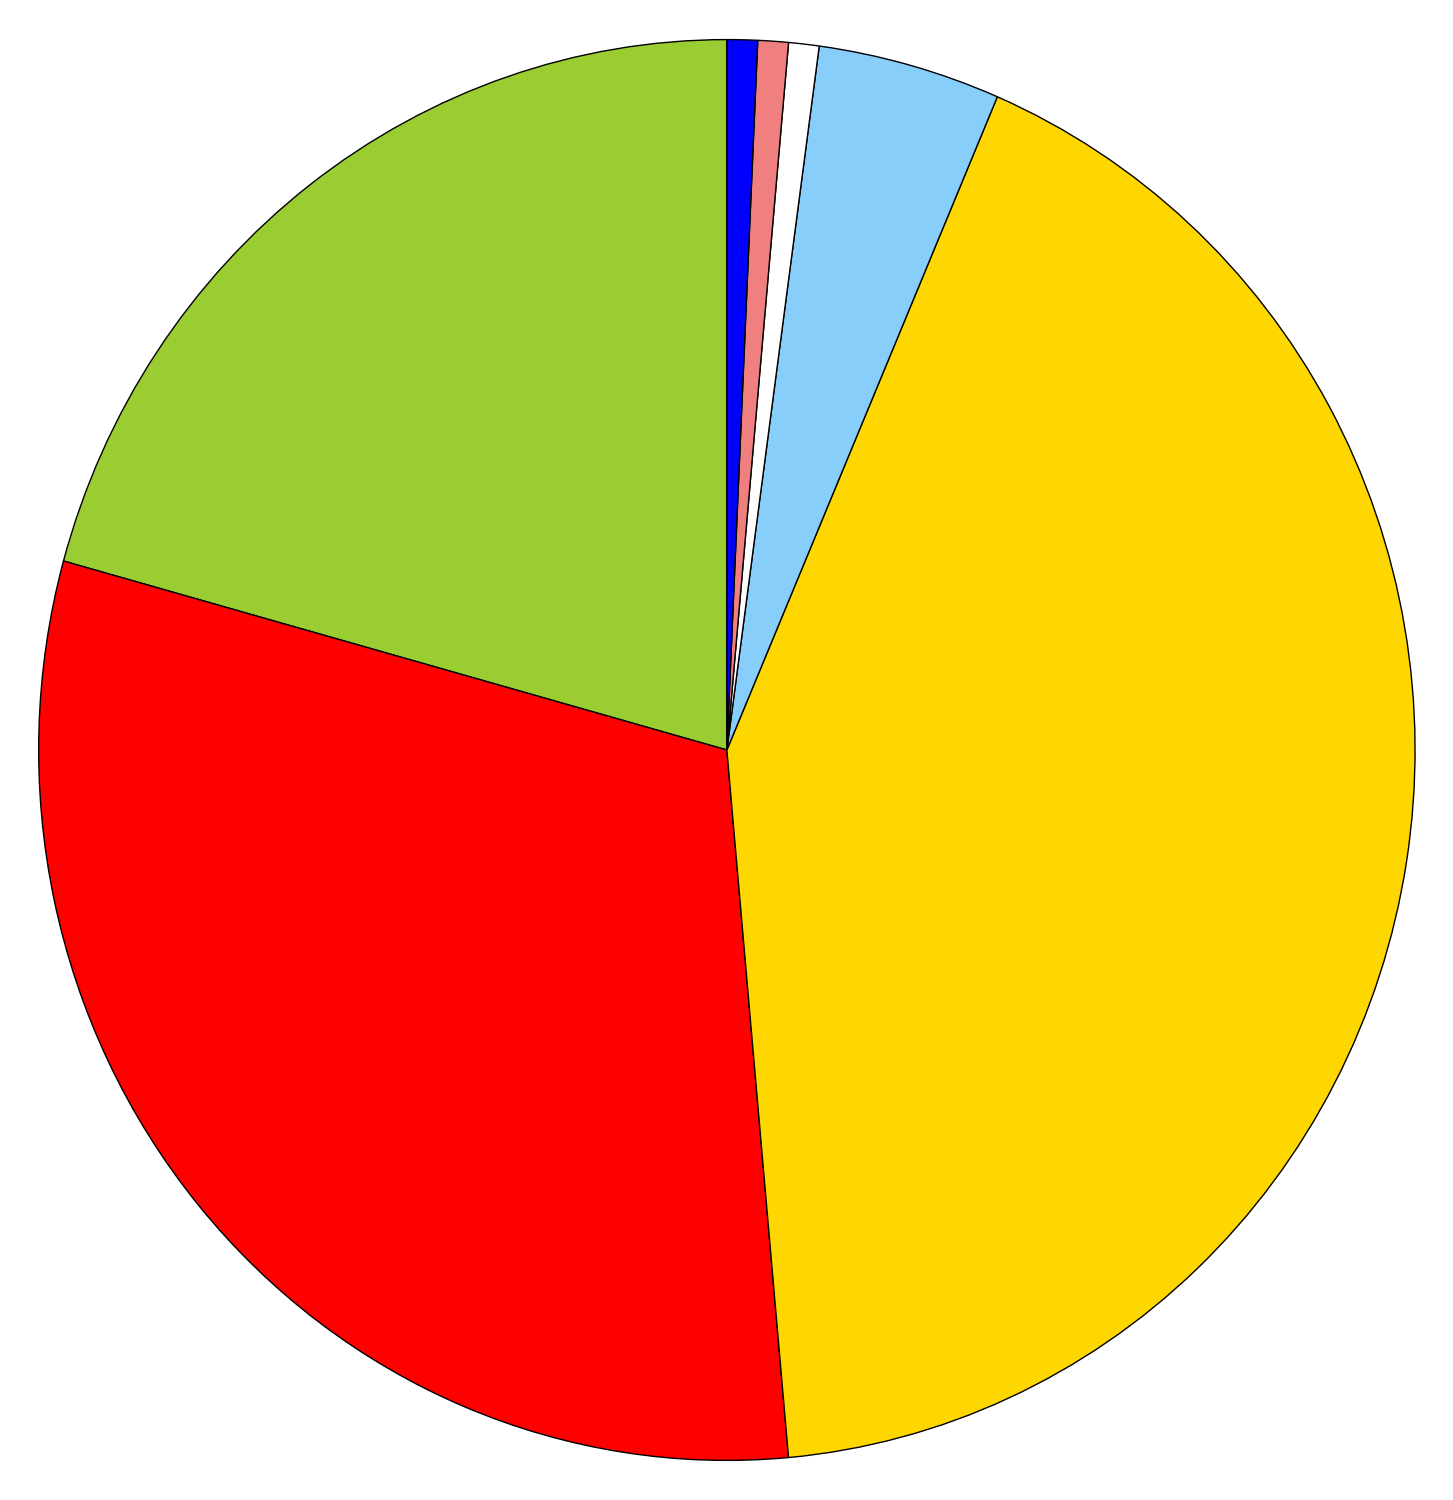
\includegraphics[width=\textwidth]{arousalALLL1}
    \caption{Lasso regression}
  \end{minipage}
  \hfill
  \begin{minipage}[b]{0.3\textwidth}
    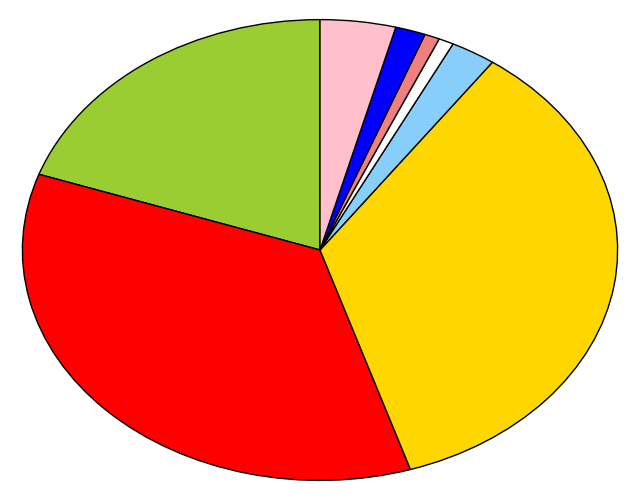
\includegraphics[width=\textwidth]{arousalALLL2}
    \caption{Ridge regression}
  \end{minipage}
  
  \begin{minipage}[b]{0.3\textwidth}
    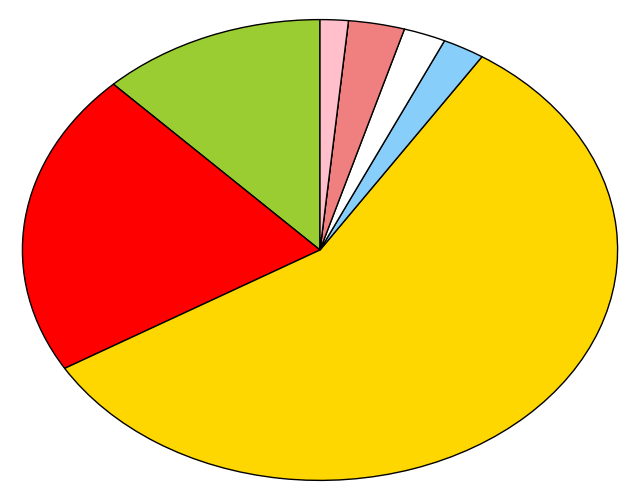
\includegraphics[width=\textwidth]{arousalALLRF}
    \caption{Random forests}
  \end{minipage}
  \hfill
  \begin{minipage}[b]{0.3\textwidth}
    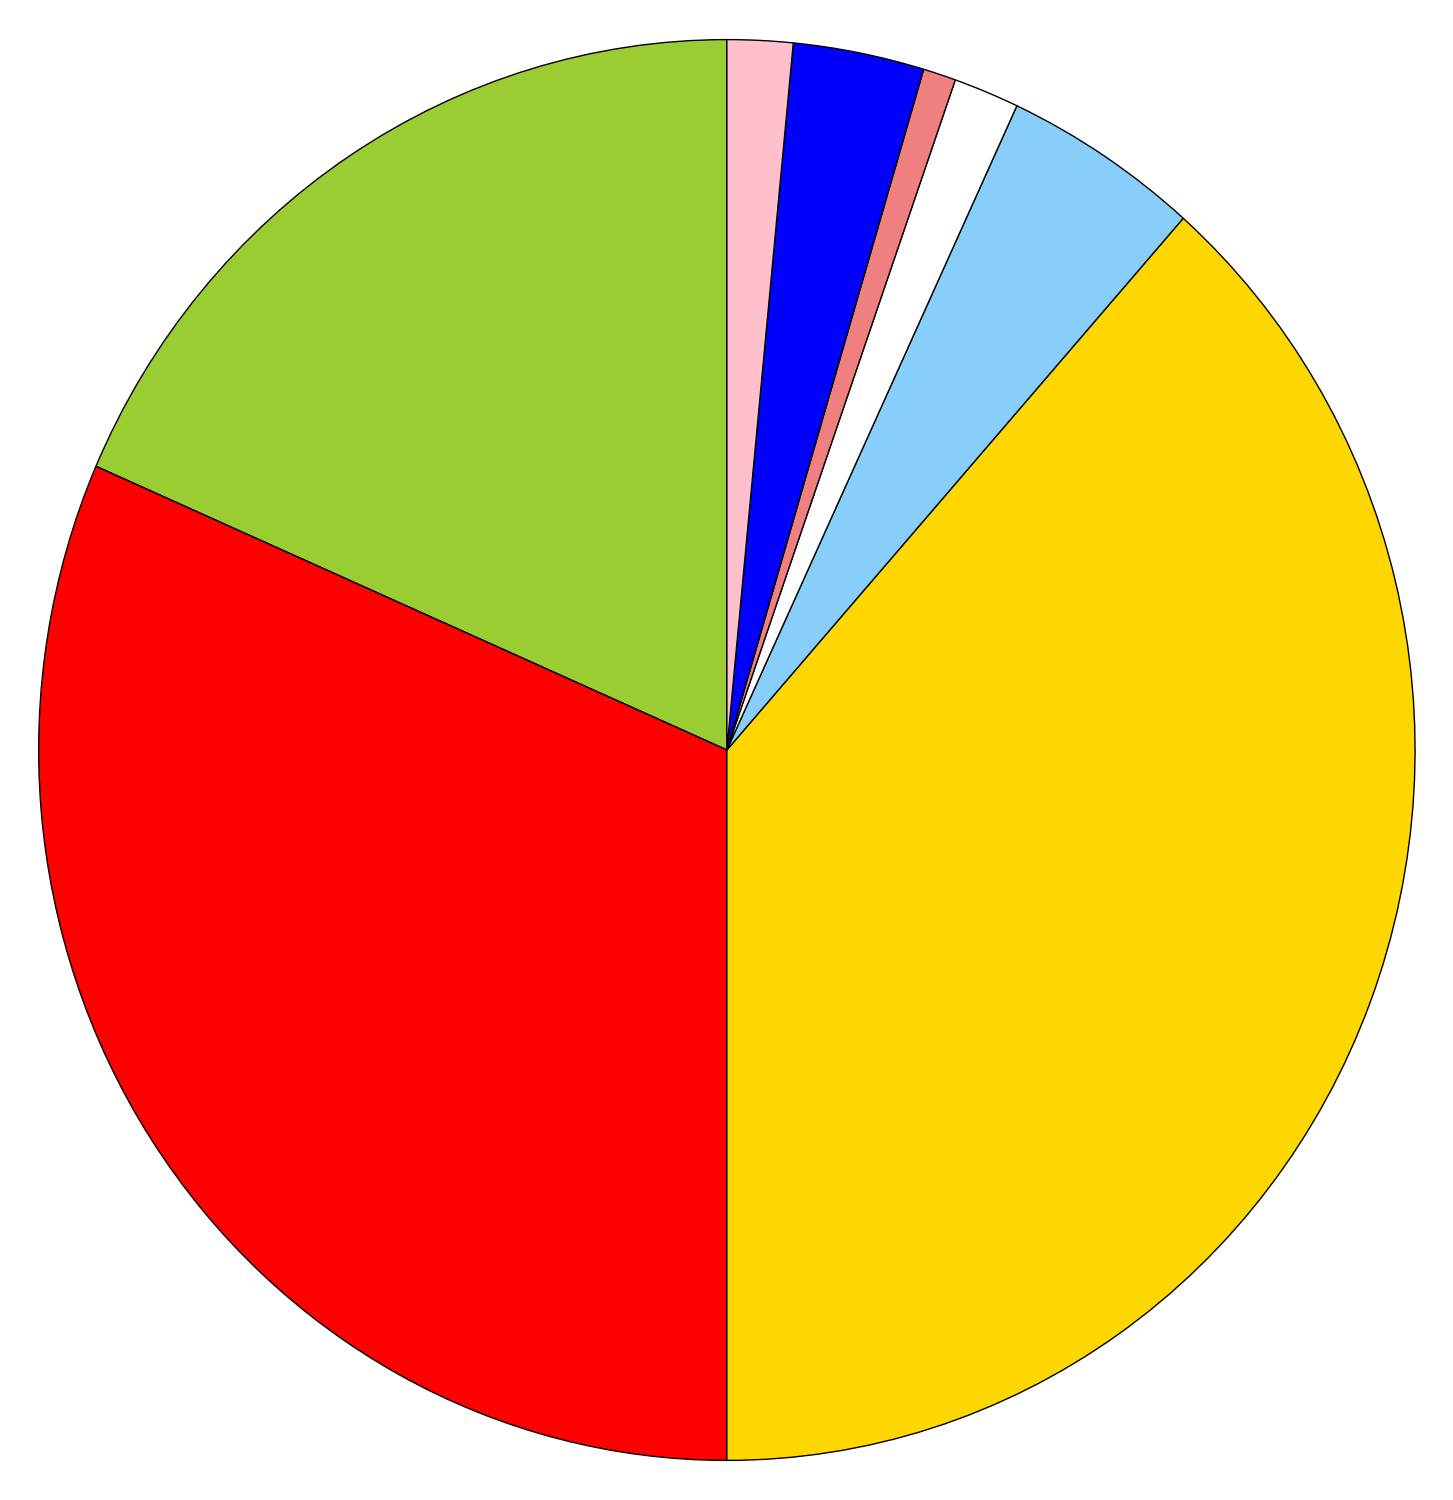
\includegraphics[width=\textwidth]{arousalALLPCA} %TODO 
    \caption{PCA}
  \end{minipage}
  \hfill
  \begin{minipage}[b]{0.3\textwidth}
    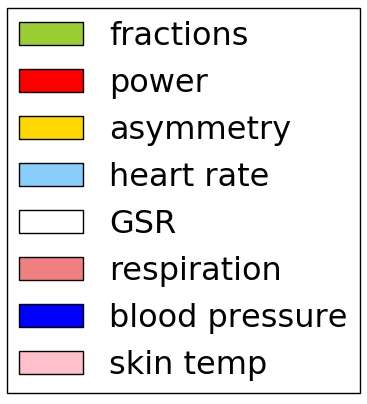
\includegraphics[width=\textwidth]{legend}
    \caption{Legend\label{arousalpieslegend}}
  \end{minipage}
\end{figure}
\clearpage




%freq table
%regions

%EEG/non-EEG/all => p value
\subsection{Certain <-> borderdist}

